\section{Trigger}
The LHC delivers proton-proton collisions at the beam crossing 
interval of 25 ns, this corresponds to a crossing frequency of 40 MHz.
Each interaction, or event, requires 0.5 to 1 megabytes of storage space.
%%%%%%%%%fix here
As it is responsible for all data acquisition, %%fix
the trigger system is the most important subsystem of CMS. 

The CMS trigger system is divided into two parts: the Level 1 trigger 
and the High Level Trigger (HLT). 
The Level 1 trigger uses coarsely segmented
data from only the calorimeters and the muon system to make initial
data selections while holding high resolution data in pipelined memories
in front-end electronics. The Level 1 Trigger hardware is implemented in customized
programmable memory look up tables (LUTs), FPGAs and asics.
The Level 1 trigger must reduce rates by at least a factor of 10$^{6}$, 
resulting in a final output of approximately 30kHz,
before high resolution data is passed to the HLT.
The HLT has access to the complete readout of the event and can use
complex algorithms to filter events. For particularly interesting events, 
the algorithms used in this process are often similar to what is done in 
offline analysis. 
  \subsection{Level 1 Trigger}
The purpose of the Level 1 trigger is to reduce rates from the input
crossing rate of 40MHz to a maximum output rate of 100kHz. 
The first step in this process is to create
calorimeter trigger primitives using a calorimeter trigger primitive generator (TPG).
For the purpose of providing compact, fast information the calorimeters
are divided into trigger towers; the TPG sums the transverse energy the
ECAL crystals or HCAL read-out towers to obtain a trigger tower E$_{T}$.
For $|\eta|<$2.1, trigger towers have a granularity
in $\eta \times \phi$ of 0.087$\times$0.087, the granularity decreases at higher
$\eta$ values. 
The TPG electronics are integrated with the calorimeter readout and the trigger primitives
are passed to the Regional Calorimeter Trigger (RCT) using
high-speed serial links.
An electron or photon candidate is expected to be narrow in $\eta$
and broader in $\phi$ therefore, an additional bit is used to indicate whether 
an electron candidate  
After that, the RCT combines tower information to form electron and 
photon candidates. The RCT also sums ECAL and HCAL towers into broader
regions which are used in the GCT to form jets. These regions also have a 
$\tau$-veto bit which determines how compatible a region is with a
$\tau$ lepton. After the GCT has combined regions to form jets, the GCT
then sorts the electron/photon candidates and jets and passes them onto
the Global Trigger.

The Muon Trigger uses all three muon systems (DTs,RPCs,CSCs) for triggering.
The DT system has excellent timing resolution and is used to reconstruct tracks
and associate tracks to bunch crossings. At a regional level, the DT and CSC track finders
combine segments to build muon tracks and assign transverse momentum using
LUTs. All regional information from the three muon systems are then forwarded
to the Global Muon Trigger (GMT) where it is then combined to proved track
information with equal or better resolution than the regional systems. The tracks
are then ranked and forwarded to the Global Trigger (GT).
  \subsection{Regional Calorimeter Trigger}
The Regional Calorimeter Trigger is responsible for level 1 triggering of the 
Electromagnetic and Hadronic calorimeters in barrel, endcap and the HF forward detector.
The RCT consists of 18 crates installed in nine racks in the CMS underground 
counting room, which is adjacent to and shielded from the CMS cavern.
For triggering purposes, the HCAL and ECAL are subdivided into regions in 
$(\eta,\phi)$. As illustrated in figure \ref{fig:rctTowerIetaIphi}
a region consists of of 4$\times$4 trigger towers; 
the RCT has 7 receiver cards per crate and one jet summary card for the 18 crates. 
A total of 24 bits is received from each trigger tower: 
two 8-bit calorimeter energies each from the ECAL and the HCAL,
two energy characterization bits, 5 bits of error detection and 1 LHC bunch crossing bit.
\begin{figure}[hb]
  \centering
	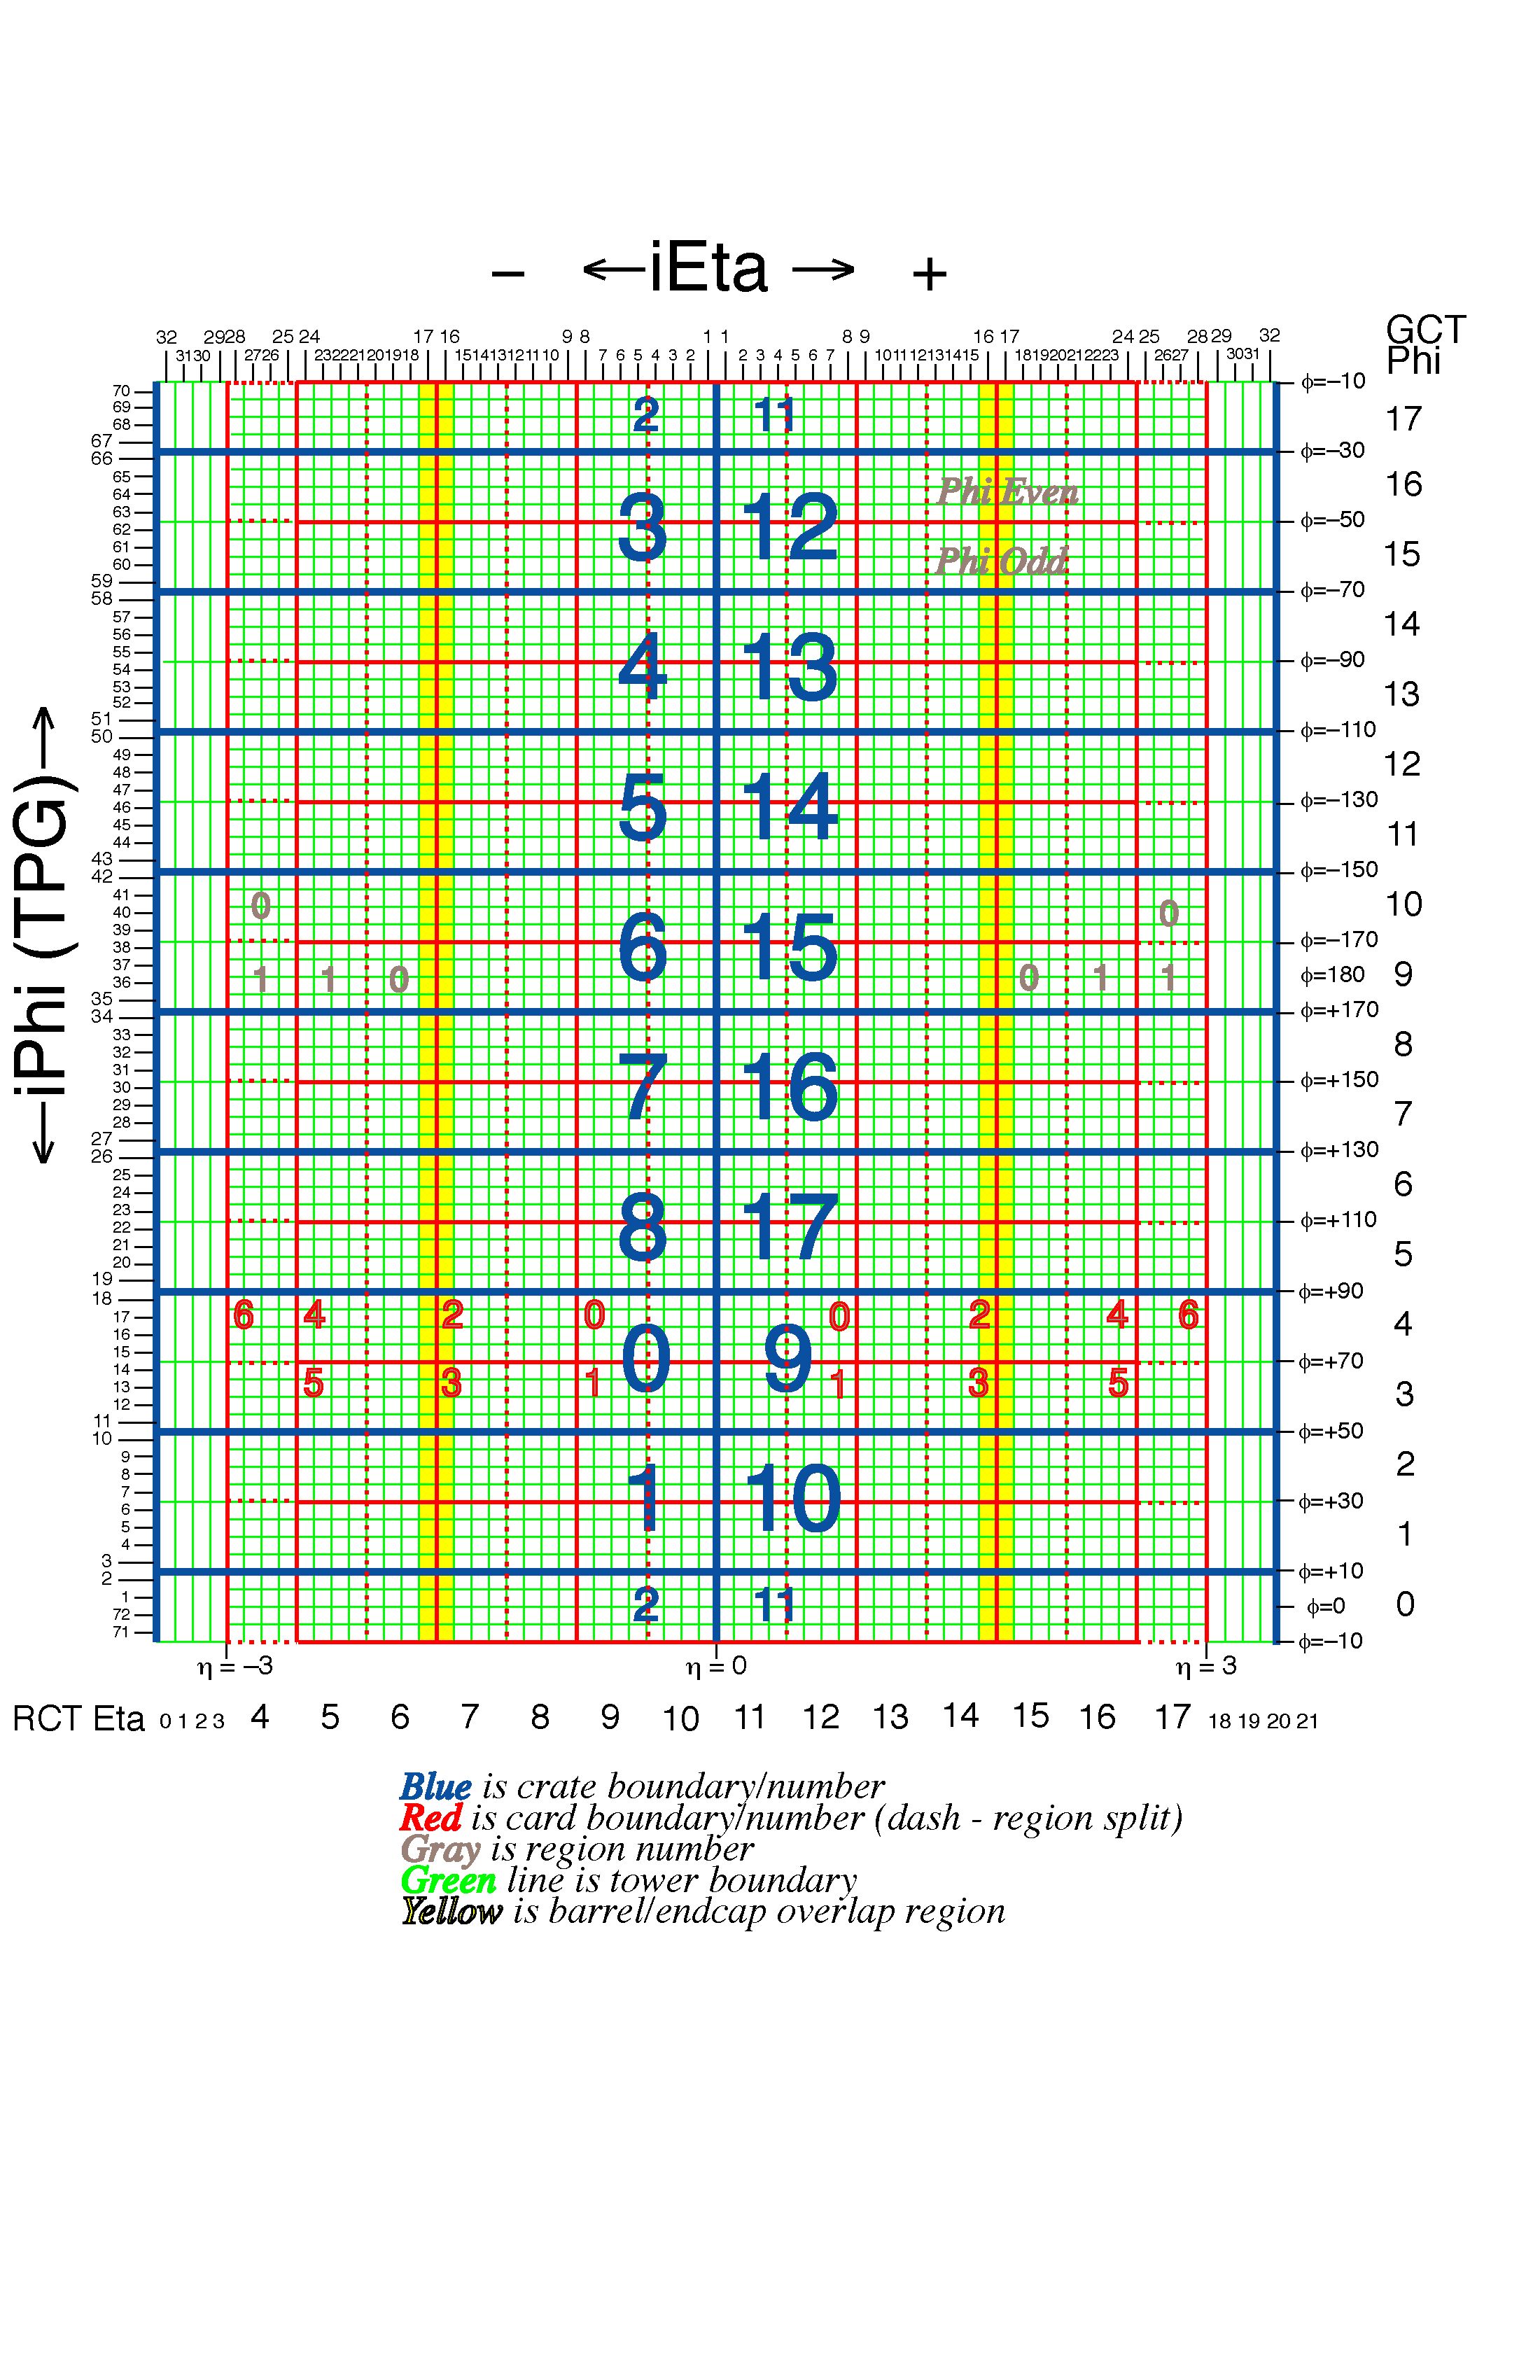
\includegraphics[trim = 0mm 80mm 0mm 42mm, clip, width=0.75\textwidth]{images/towers_ieta_iphi.png}
  	\caption[RCT Layout]
   	{RCT layout}
	\label{fig:rctTowerIetaIphi}
\end{figure}

Good $e/\gamma$ selection efficiency at a low rate is essential. $e/\gamma$
identification in the RCT takes place as follows: starting from the trigger towers
the RCT sums of ECAL and HCAL energies and also calculates the
the ratio of HCAL to ECAL energy, $(H/E)$. The $(H/E)$ ratio is used to
discriminate electrons and photons from pions and electromagnetic deposits
in jets. 
The RCT $e/\gamma$ algorithm is applied to ECAL trigger towers that have an energy
higher than their four immediate neighbors. The seeding tower must also 
have an energy deposit which is contained within 2$\times$5 crystals, 
this is known as the fine grain requirement and, if this is true,
a fine grain bit is set by the TPGs. 
Then, the tower energy is combined with the nearest highest energy neighbor,
this accounts for particles that deposit energy in two towers; this sum is then
associated with the $e/\gamma$ candidate.
To further separate from jets, the RCT also determines if the $e/\gamma$ candidate
is isolated. As can be seen in figure \ref{fig:emRCTalgo}.
\begin{figure}[hb]
  \centering
	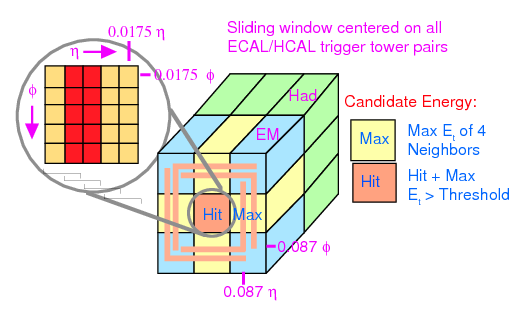
\includegraphics[width=0.75\textwidth]{images/emRCTalgo.png}
  	\caption[e/$\gamma$ Fine Grain and Isolation]
   	{The fine grain veto bit is set if an $e/\gamma$ deposit is not contained
	within a 2$\times$5 ECAL crystal area (as can be seen in red). An Isolated
	electron is required to have a at least twi of the L-Shaped corners (in tan) 
	to below a certain threshold}
	\label{fig:emRCTalgo}
\end{figure}
the 8 towers around the central are divided into L-shaped quiet corners,
for an electron to be considered isolated two of these must have an energy
below a configurable threshold; those towers must also not have the fine grain
bit set.
The RCT then ranks the isolated and the non-isolated $e/\gamma$ candidates
and passes the highest four to the GCT. These collections of isolated and non-isolated
candidates are mutually exclusive. Due to having a sufficiently low rate, all isolated
and electrons with a transverse momentum greater than 63.5 GeV
are accepted as isolated for the 2011 and 2012 runs. 

\begin{figure}[hb]
  \centering
	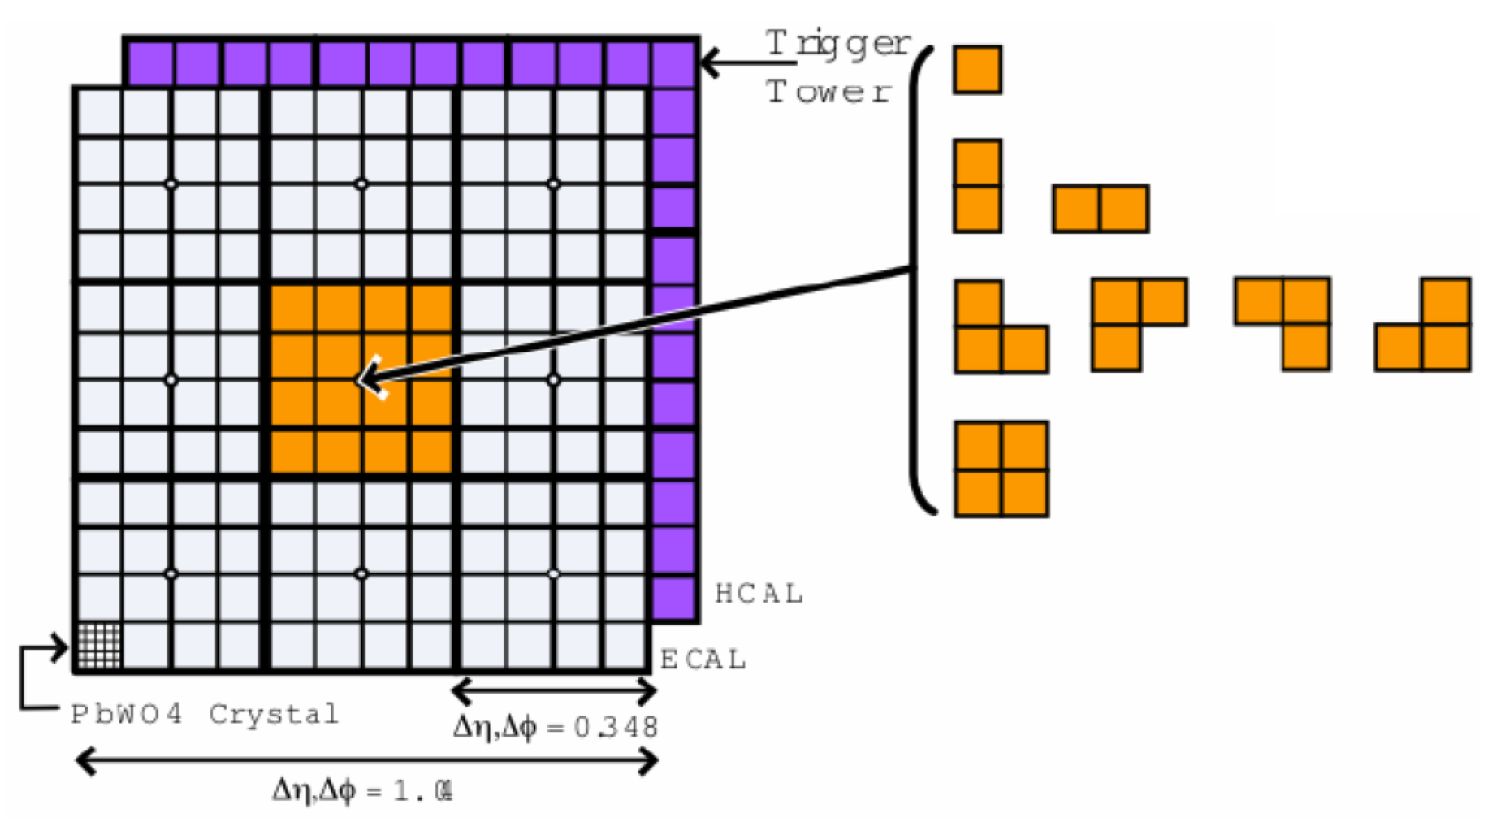
\includegraphics[width=0.75\textwidth]{images/RCTTauAlgo.png}
  	\caption[RCT Tau ID Algorithm]
   	{RCT Tau Identification Algorithm}
	\label{fig:RCTTauAlgo}
\end{figure}
For the purpose of jet reconstruction, the RCT also sums ECAL and HCAL 
energies in clusters of 4$\times$4 towers (as can be seen in figure \ref{fig:rctTowerIetaIphi}
) in to regions. During this process the RCT examines the
energy profile to see if the region is compatible with a hadronic $\tau$ lepton.
A $\tau$-veto bit is set unless the pattern of active towers corresponds to at
most 2$\times$2 contiguous towers. The patterns are detailed in figure \ref{fig:RCTTauAlgo}
This $\tau$ veto bit is included when the jet transverse energy is sent to the GCT.
The RCT is an essential system for data acquisition at a high efficiency and
a low rate, therefore good performance must be continually monitored during and
between runs.
Using the RCT emulator, the performance of the RCT is monitored during 
and after data-taking by constantly comparing the trigger 
output with the expected output from the RCT Emulator. The RCT data quality monitoring 
software package runs the RCT emulator on a subset of events and compares
the emulator response with the hardware response for each event.

%A calibration factor that is measured offline as a function of 
%$\eta$ is stored in the Look-Up tables and applied to the electron/photon candidates.
  \subsection{High Level Trigger}
After events pass the Level 1 trigger they are sent to the High Level Trigger (HLT). The
HLT uses a filter farm of processors to reduce rates by a factor of 10$^{6}$ from 
100 kHz to a final output rate of less than 300 Hz. This filter farm takes as input
data that is processed by the Data Acquisition (DAQ) system. The DAQ system is responsible
for taking data which is pushed into the DAQ by Front-End Drivers (FEDs) at a maximum input 
rate of 100kHz which corresponds to a data flow of $\approx$100 GByte/s from approximately
650 data sources. An event builder assembles the event fragments from all FEDs
which belong to the same Level 1 output; this data is then sent from underground to the surface %%%change
building, SCX where the HLT is located.
Algorithms for data selection are implemented in the HLT are written in
C++ and are similar to or exactly the same as algorithms that are used in offline selection. This 
further helps to ensure a high efficiency of interesting physics events.
The HLT processing time depends primarily on the algorithm complexity,
therefore, simple algorithms are processed first and if an event fails a selection
step then a node is free for the next event.
